\DocumentMetadata{
  pdfversion=2.0,
  lang=es-MX,
  pdfstandard=ua-2
}

\documentclass{sener2025}

\addbibresource{referencias.bib}

% --- Metadatos PDF/UA (Accesibilidad Universal) ---
\hypersetup{
  pdftitle={Documento DEMO — Plantilla SENER LaTeX},
  pdfauthor={Equipo de Planeación (demo)},
  pdfsubject={Ejemplos de secciones, etiquetas y bloques (para pruebas del generador)},
  pdfkeywords={demo; plantilla; secciones; etiquetas; tablas; figuras},
  pdfcreationdate={D:20251216121138},
  pdfversion={1}
}

% --- Metadatos del Documento ---
\title{Documento DEMO — Plantilla SENER LaTeX}
\subtitle{Ejemplos de secciones, etiquetas y bloques (para pruebas del generador)}
\author{Equipo de Planeación (demo)}
\date{14 de diciembre de 2025}
\institucion{Secretaría de Energía (SENER)}
\unidad{Unidad de Planeación y Transición Energética}
\setDocumentoCorto{DEMO\_SENER\_SASSO}
\palabrasclave{demo; plantilla; secciones; etiquetas; tablas; figuras}
\version{1}

\begin{document}

\portadafondo[img/portada.png]

\tableofcontents
\newpage

\listafiguras
\newpage

\listatablas
\newpage

\clearpage
\begin{center}
{\Large\patriafont\bfseries\color{gobmxGuinda}Agradecimientos}\\[1cm]
\end{center}

Agaredecemos a:
1.-JAvi
2.-Diego
3.-Rodrigo

\clearpage
\begin{center}
{\Large\patriafont\bfseries\color{gobmxGuinda}Presentación}\\[1cm]
\end{center}

ESto es un texot de presemntacion ..... bka....bla...blan

\clearpage
\begin{center}
{\Large\patriafont\bfseries\color{gobmxGuinda}Resumen Ejecutivo}\\[1cm]
\end{center}

Este documento es un banco de pruebas. Incluye ejemplos de:
• Listas
• Etiquetas inline (nota, cita, math)
• Bloques (recuadro, ejemplo, info, alerta)
• Anexos
• Tablas y figuras

Objetivo: detectar errores de escape y de parsing antes de publicar.

\clearpage
\begin{center}
{\Large\patriafont\bfseries\color{gobmxGuinda}Datos Clave}\\[1cm]
\end{center}

\begin{itemize}
  \item Dato 1
  \item Dato 2
  \item Dato 3
  \item Dato 4
\end{itemize}

\portadaseccion{1}{Capítulo 1}{Guía rápida (etiquetas + bloques)}

\section{Guía rápida de sintaxis}

Este párrafo muestra texto normal con acentos (México, energía, transición).
También prueba caracteres especiales que deben escaparse: 100\% , \$1,234 , \& , \_ , \# , \{ \} .

Ejemplo de nota al pie: La demanda eléctrica crece de forma sostenida\footnote{Nota al pie desde Sheets/Excel. Soporta texto largo y símbolos como \% y \&.}.
Ejemplo de cita bibliográfica: ver \cite{demo_sener2025} y \cite{cenace2023_flex}.

Inline math: El coeficiente de potencia es $C_p$ y la eficiencia $\eta = \frac{P_{out}}{P_{in}}$.
Display equation (sin escapar comandos dentro):
\begin{equation}
\eta = \frac{P_{out}}{P_{in}}
\end{equation}

Lista simple (una línea = un item):
\begin{itemize}
  \item Primer punto con \textbf{\textcolor{gobmxDorado}{énfasis dorado}}
  \item Segundo punto con \textbf{\textcolor{gobmxGuinda}{énfasis guinda}}
  \item Tercer punto con referencia a tabla/figura (opcional): [[tabla:capacidad]] y [[figura:capacidad]]
\end{itemize}
Prueba de saltos como texto literal: escribe

 en una celda y asegúrate que el pipeline lo convierta en salto real (esto es un test).


\subsection{Etiquetas inline (dentro de un párrafo)}

Puedes mezclar etiquetas dentro de texto:
\begin{itemize}
  \item \textbf{\textcolor{gobmxDorado}{Texto dorado}} y \textbf{\textcolor{gobmxGuinda}{Texto guinda}}
  \item Nota al pie: \footnote{Una nota corta.}
  \item Citas: \cite{demo_sener2025}
  \item Math inline: $E = mc^2$
\end{itemize}
Recomendación: usa estas etiquetas inline SOLO para fragmentos cortos. Para cajas completas usa bloques.


\subsection{Bloques (cajas) usando líneas separadas}

Los bloques deben ir en líneas separadas, así:

\begin{recuadro}[title={Nota metodológica}]
Este recuadro acepta varias líneas.
También acepta listas:
\begin{itemize}
  \item Item A
  \item Item B con \textbf{\textcolor{gobmxDorado}{resaltado}}
\end{itemize}
\end{recuadro}

\begin{ejemplo}[title={Ejemplo de cálculo}]
Si P es potencia y V voltaje, entonces:
\begin{equation}
P = V\cdot I
\end{equation}

\end{ejemplo}

\begin{calloutTip}
Tip: usa $\Delta$ para deltas y $\%$ no es necesario (el generador debe escapar \% en texto normal).

\end{calloutTip}

\begin{calloutWarning}
Advertencia: si escribes comandos LaTeX crudos (\textbackslash\{\}begin, \textbackslash\{\}textbf, etc.) el generador los escapará a menos que tengas una etiqueta especial para 'raw'.

\end{calloutWarning}


\section{Tablas y figuras (inserción automática)}

Esta sección está pensada para probar que el generador inserta automáticamente:
\begin{itemize}
  \item 1 figura asociada con SeccionOrden=2.0 (ver hoja 'Figuras').
  \item 2 tablas asociadas con SeccionOrden=2.0 (ver hoja 'Tablas' y rangos en 'Datos Tablas').
\end{itemize}
Si quieres referenciar explícitamente en texto, puedes poner comentarios:
% Referencia a figura: Figura 2.1
% Referencia a tabla: Tabla 2.1
\begin{figure}[H]
  {\centering
  % Texto alternativo para accesibilidad
  \pdftooltip{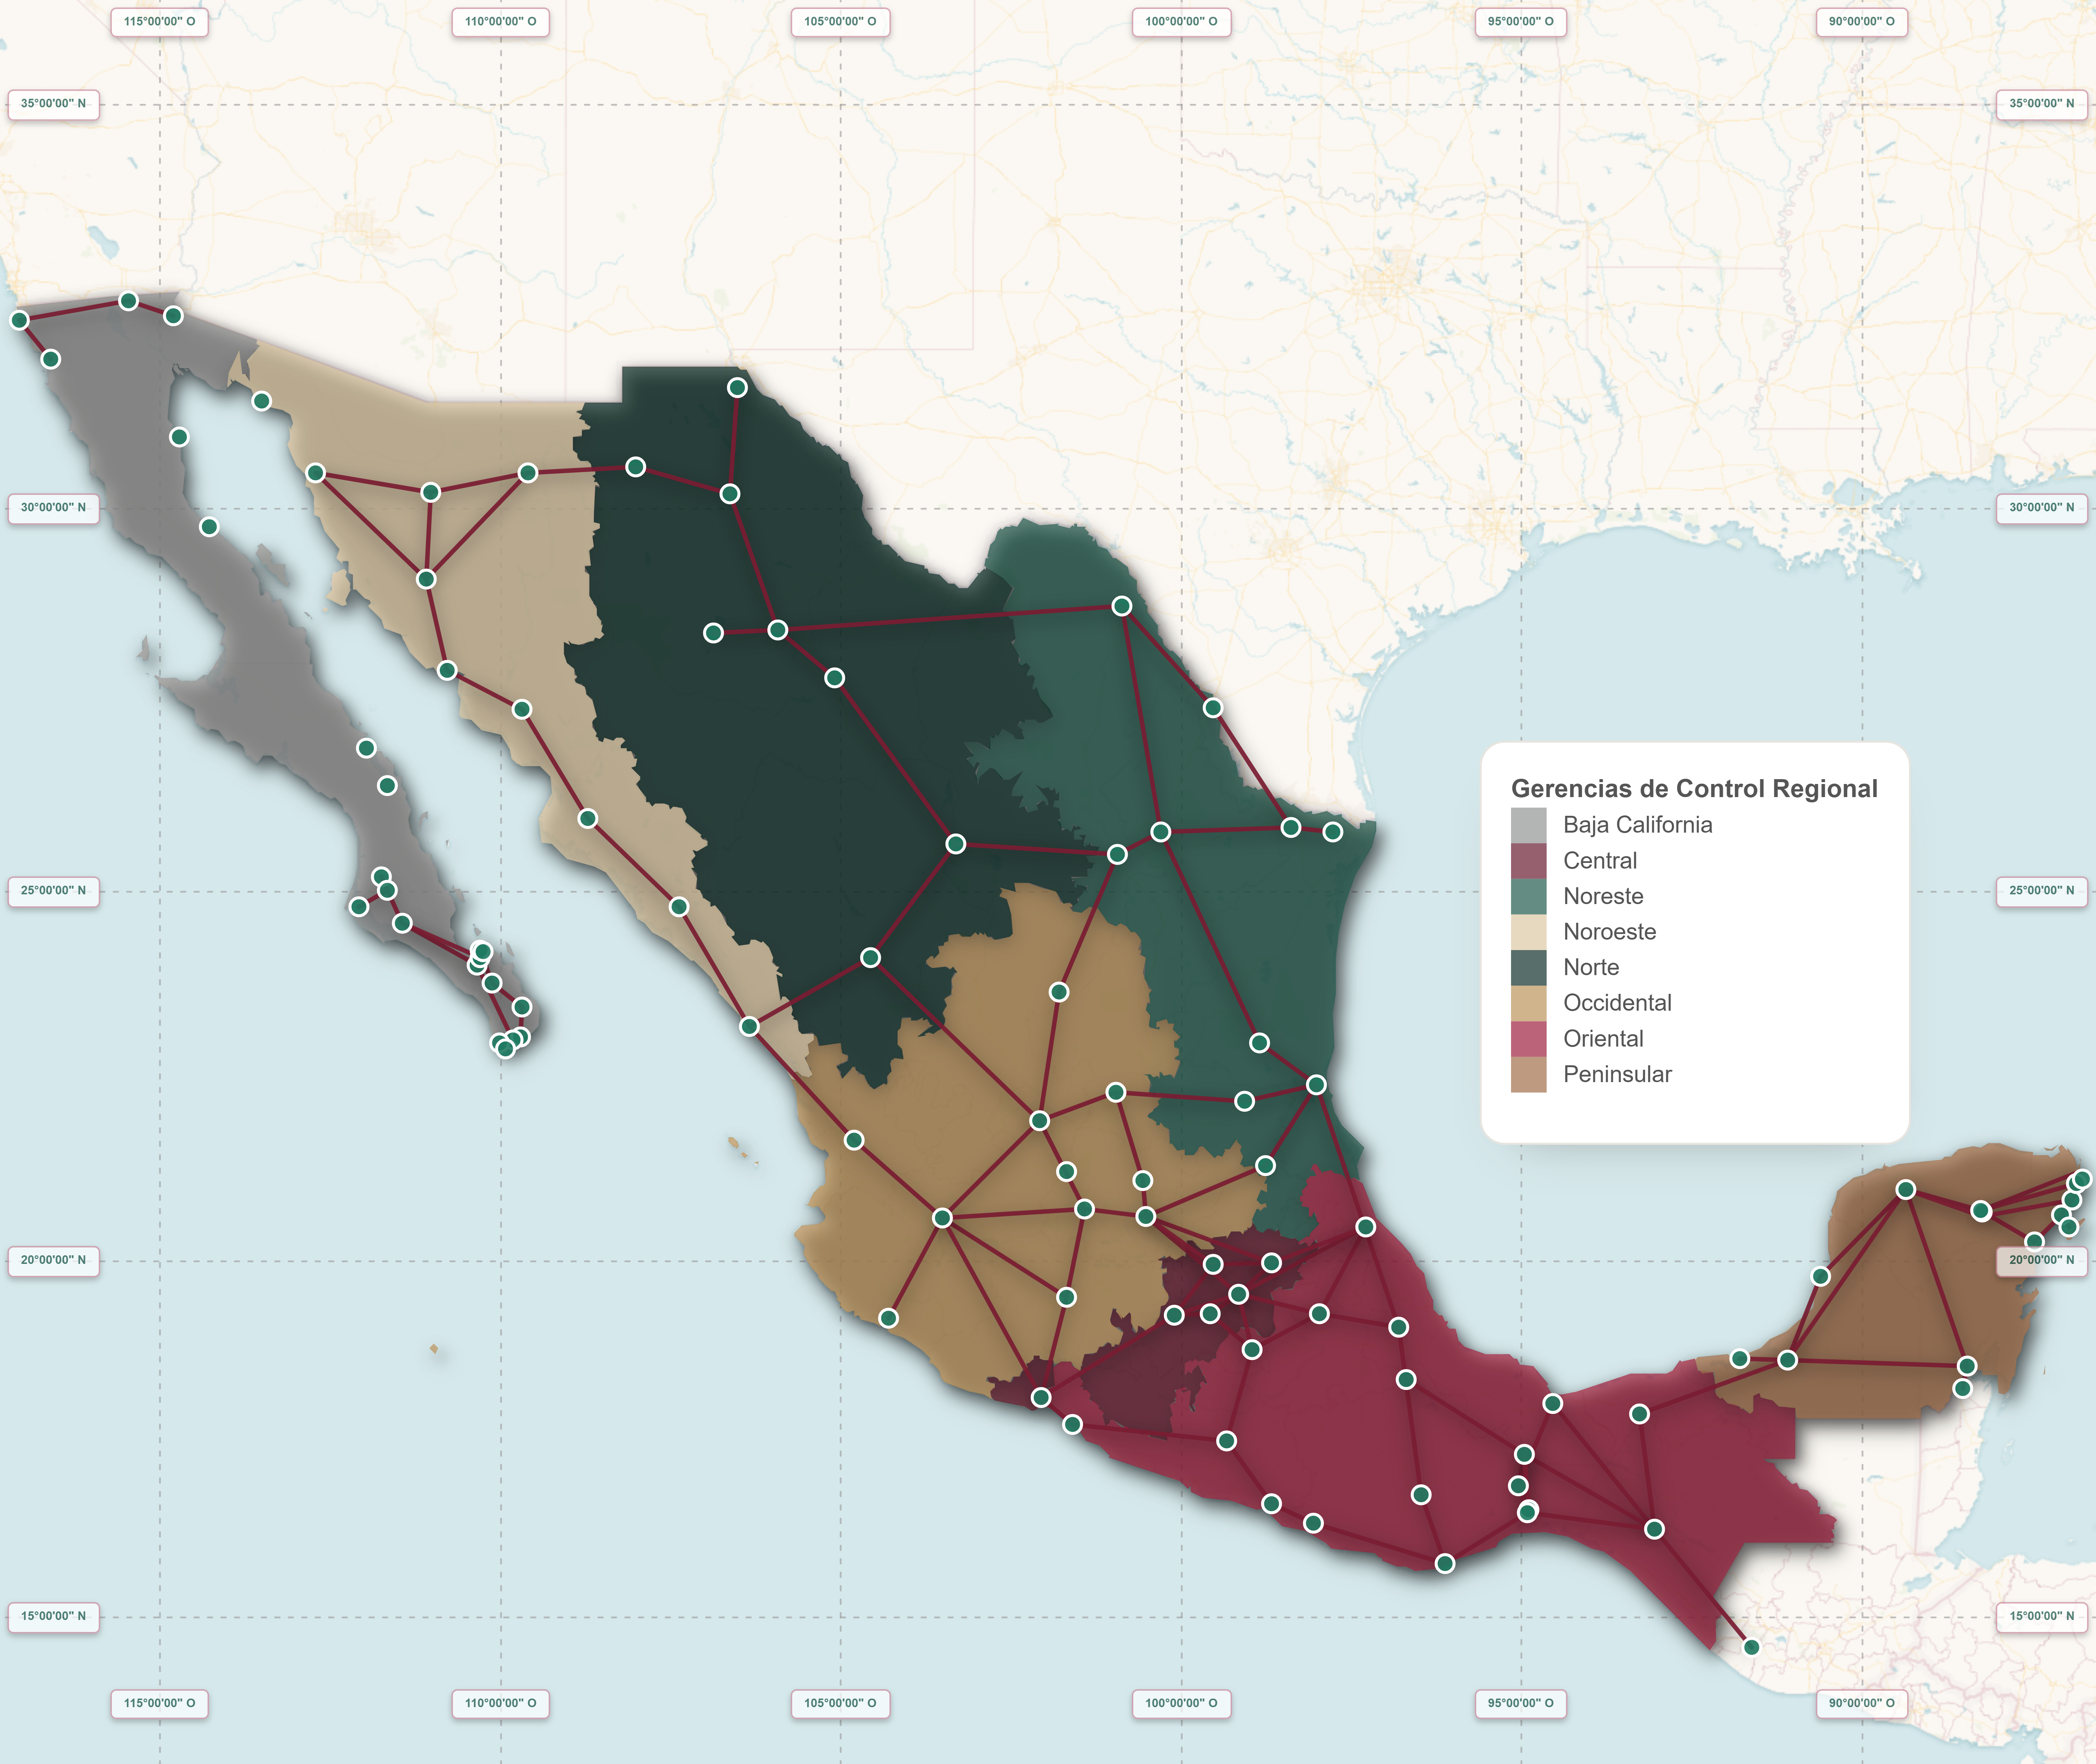
\includegraphics[width=0.8\textwidth]{img/graficos/figura_2_1.png}}{Gráfica circular (pie chart) que muestra la distribución porcentual xy del consumo energético en México por sector económico durante 2024. Sector industrial: 45\% (color guinda), sector transporte: 30\% (verde), sector residencial: 15\% (dorado), otros sectores: 10\% (gris). Total: 100\% equivalente a 4,250 petajoules.}
  \par}
  \raggedright
  \caption{Evolución de la capacidad instalada por tecnología, 2020–2025s}
  \label{fig:evolucion_de_la_capacidad_inst}
\end{figure}
\vspace{-4pt}
\fuente{SENER,2025}

\begin{tabladoradoCorto}
  \caption{Tabla demo (corta): Capacidad por tecnología}
  \label{tab:tabla_demo__corta___capacidad_}
  \begin{tabular}{H{3cm}G{2cm}G{2cm}}
    \toprule
    \rowcolor{gobmxDorado} \encabezadodorado{\textbf{Tecnología}} & \encabezadodorado{Capacidad (MW)} & \encabezadodorado{Participación (\%)} \\
    \midrule
    \textbf{Solar FV} & 12,500 & 18.5 \\
    \textbf{Eólica} & 16,000 & 23.7 \\
    \bottomrule
  \end{tabular}
\end{tabladoradoCorto}
\vspace{-4pt}
\fuente{Elaboración propia (demo)}

\begin{tabladoradoLargo}
  \begin{longtable}{B{3cm}p{2.20cm}p{2.20cm}p{2.20cm}p{2.20cm}p{2.20cm}}
    \caption{Tabla demo (larga): Serie histórica (25 filas)}\label{tab:tabla_demo__larga___serie_hist}\\
    \toprule
    \rowcolor{gobmxDorado} \encabezadodorado{\textbf{Año}} & \encabezadodorado{Solar (MW)} & \encabezadodorado{Eólica (MW)} & \encabezadodorado{Hidro (MW)} & \encabezadodorado{CC (MW)} & \encabezadodorado{Total (MW)} \\
    \midrule
    \endfirsthead

    \multicolumn{6}{l}{\small\textit{Continuación...}} \\
    \toprule
    \rowcolor{gobmxDorado} \encabezadodorado{\textbf{Año}} & \encabezadodorado{Solar (MW)} & \encabezadodorado{Eólica (MW)} & \encabezadodorado{Hidro (MW)} & \encabezadodorado{CC (MW)} & \encabezadodorado{Total (MW)} \\
    \midrule
    \endhead

    \midrule
    \multicolumn{6}{r}{\small\textit{Continúa en la siguiente página...}} \\
    \endfoot

    \bottomrule
    \endlastfoot

    2,000 & 940 & 905 & 910 & 1,385 & 4,140 \\
    2,001 & 980 & 960 & 920 & 1,420 & 4,280 \\
    2,002 & 1,020 & 1,015 & 930 & 1,455 & 4,420 \\
    2,003 & 1,060 & 1,070 & 940 & 1,490 & 4,560 \\
    2,004 & 1,100 & 1,125 & 950 & 1,525 & 4,700 \\
    2,005 & 1,140 & 1,180 & 960 & 1,560 & 4,840 \\
    2,006 & 1,180 & 1,235 & 970 & 1,595 & 4,980 \\
    2,007 & 1,220 & 1,290 & 980 & 1,630 & 5,120 \\
    2,008 & 1,260 & 1,345 & 990 & 1,665 & 5,260 \\
    2,009 & 1,300 & 1,400 & 1,000 & 1,700 & 5,400 \\
    2,010 & 1,340 & 1,455 & 1,010 & 1,735 & 5,540 \\
    2,011 & 1,380 & 1,510 & 1,020 & 1,770 & 5,680 \\
    2,012 & 1,420 & 1,565 & 1,030 & 1,805 & 5,820 \\
    2,013 & 1,460 & 1,620 & 1,040 & 1,840 & 5,960 \\
    2,014 & 1,500 & 1,675 & 1,050 & 1,875 & 6,100 \\
    2,015 & 1,540 & 1,730 & 1,060 & 1,910 & 6,240 \\
    2,016 & 1,580 & 1,785 & 1,070 & 1,945 & 6,380 \\
    2,017 & 1,620 & 1,840 & 1,080 & 1,980 & 6,520 \\
    2,018 & 1,660 & 1,895 & 1,090 & 2,015 & 6,660 \\
    2,019 & 1,700 & 1,950 & 1,100 & 2,050 & 6,800 \\
    2,020 & 1,740 & 2,005 & 1,110 & 2,085 & 6,940 \\
    2,021 & 1,780 & 2,060 & 1,120 & 2,120 & 7,080 \\
    2,022 & 1,820 & 2,115 & 1,130 & 2,155 & 7,220 \\
    2,023 & 1,860 & 2,170 & 1,140 & 2,190 & 7,360 \\
    2,024 & 1,900 & 2,225 & 1,150 & 2,225 & 7,500 \\
    2,025 & 1,940 & 2,280 & 1,160 & 2,260 & 7,640 \\
  \end{longtable}
\end{tabladoradoLargo}
\vspace{-4pt}
\fuente{Elaboración propia (demo) Nota: tabla larga para probar longtable}



\section{Prueba de párrafos y saltos de línea}

Este es el párrafo 1.

Este es el párrafo 2 (separado por una línea en blanco).

Ahora una lista:
\begin{itemize}
  \item Línea 1
  \item Línea 2
\end{itemize}
Fin.
\begin{figure}[H]
  {\centering
  % Texto alternativo para accesibilidad
  \pdftooltip{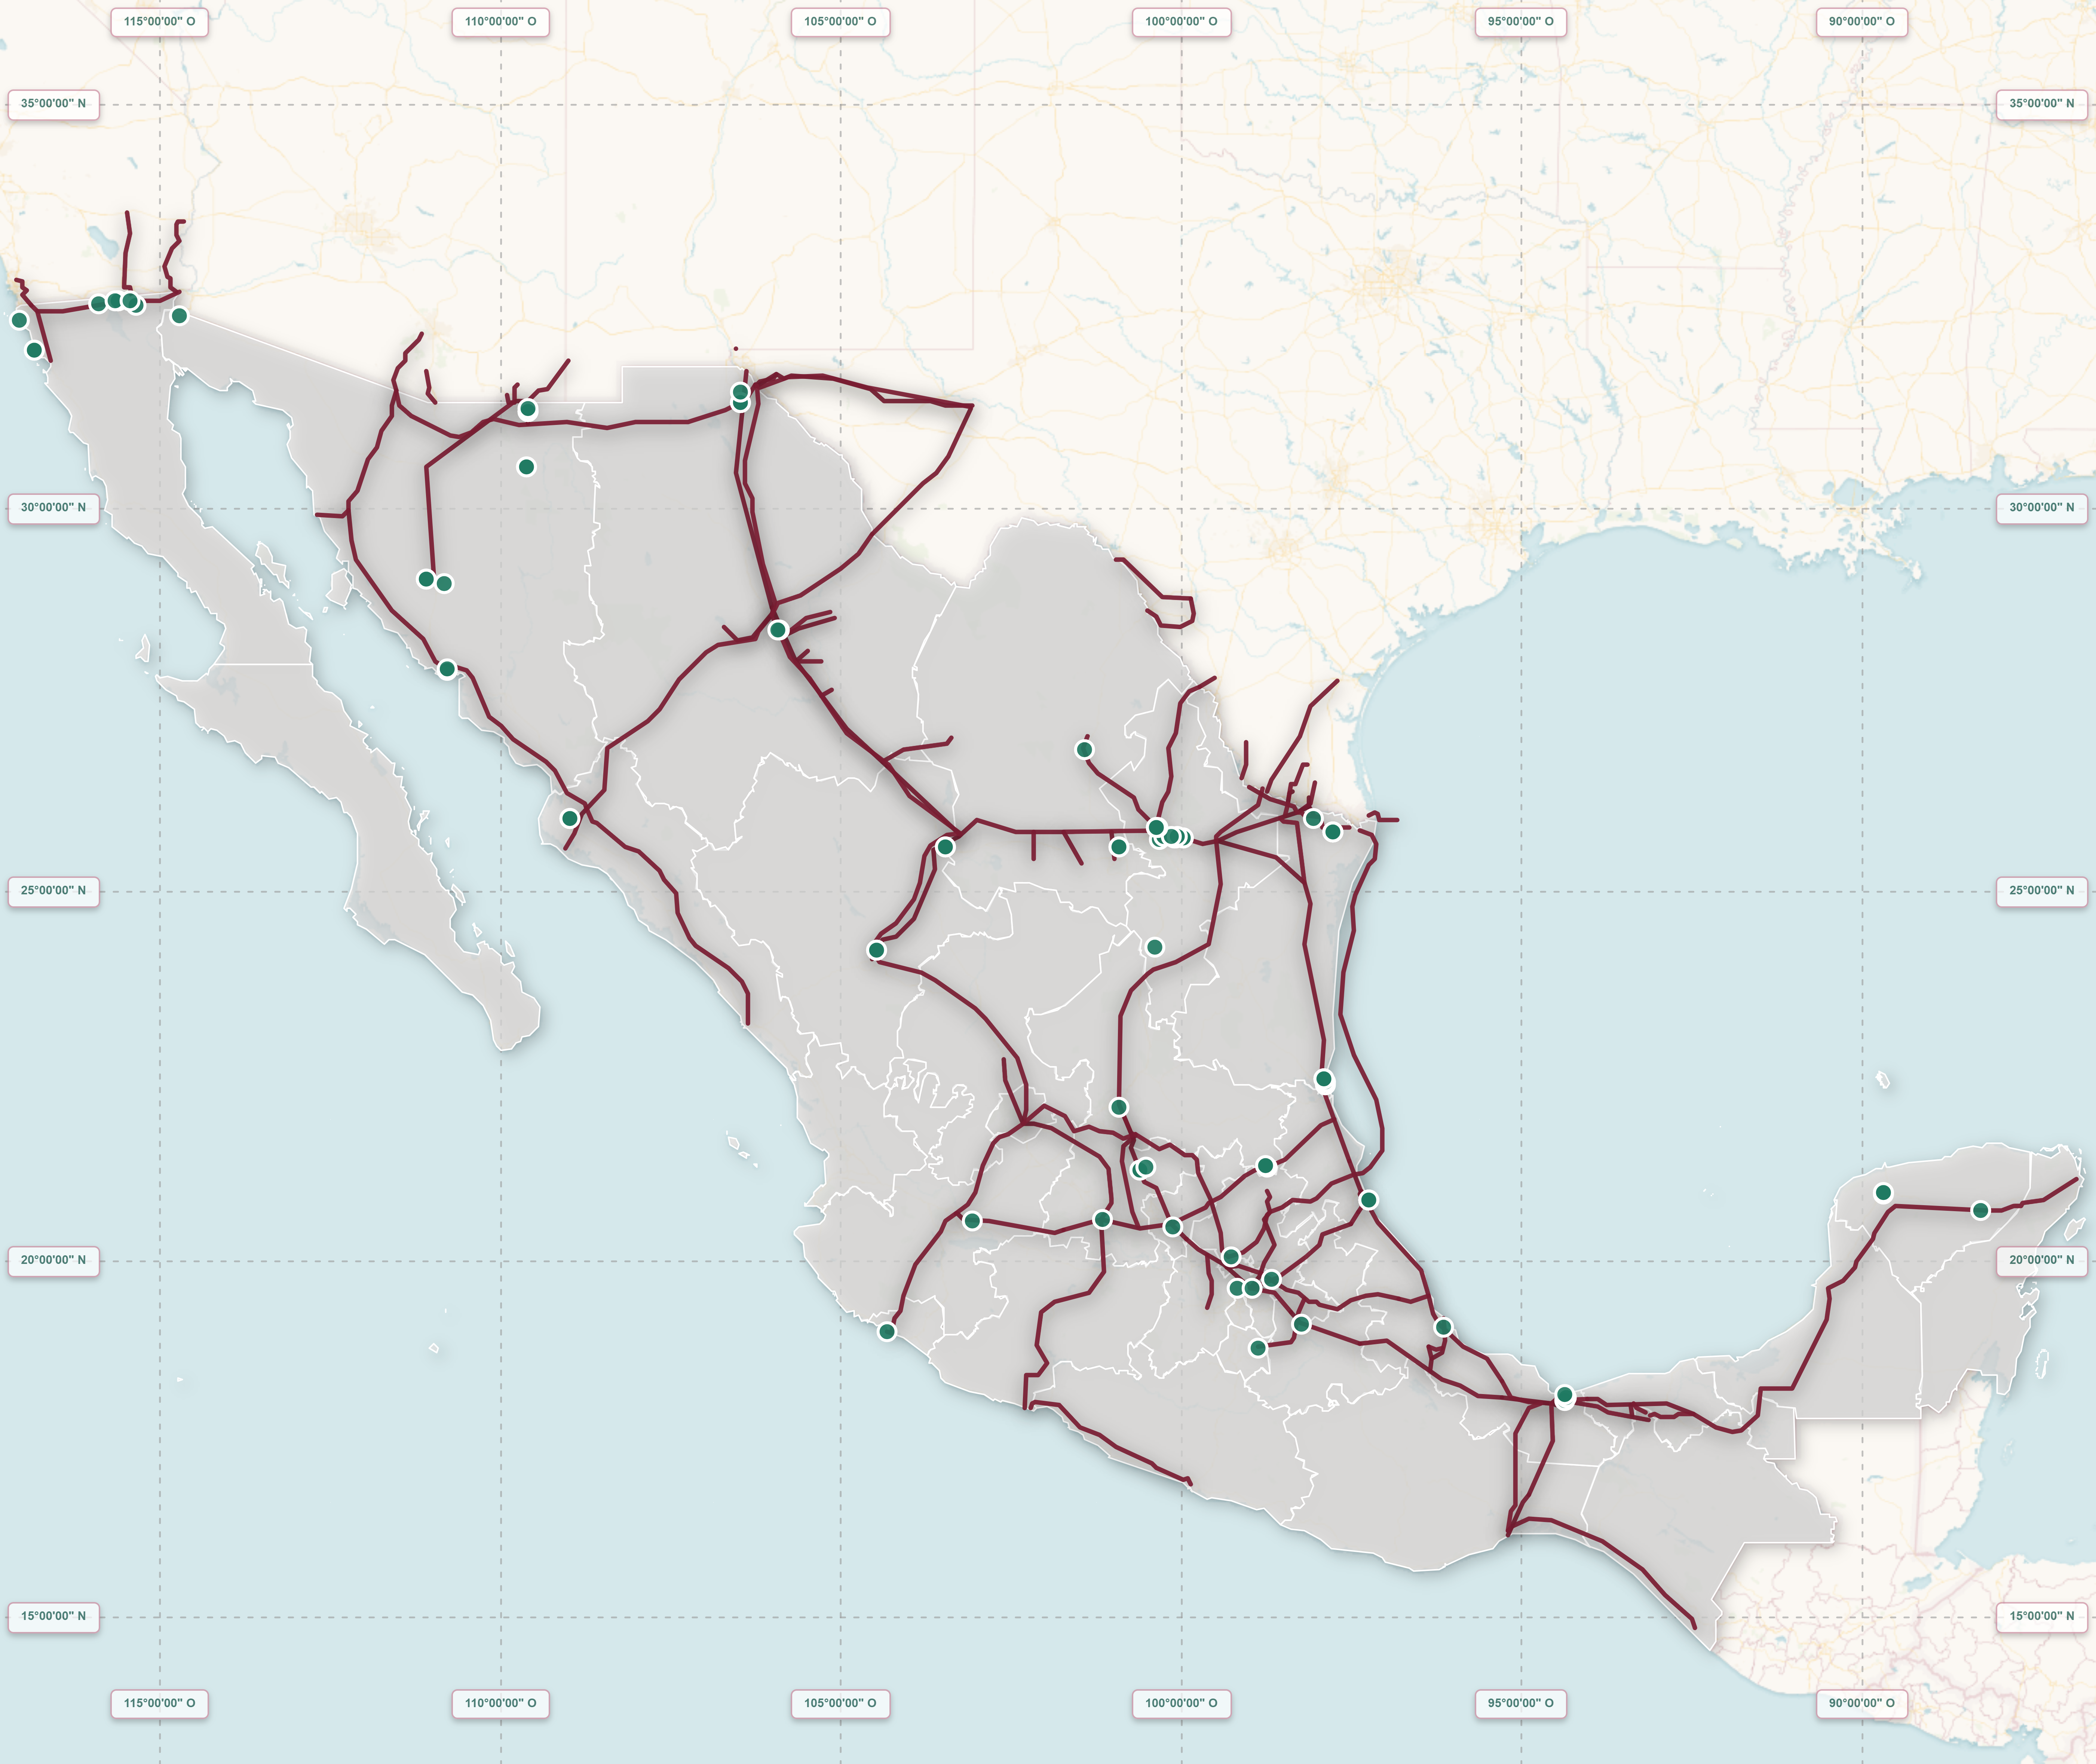
\includegraphics[width=0.8\textwidth]{img/graficos/figura_2_12.png}}{Gráfica circular (pie chart) que muestra la distribución porcentual del consumo energético en México por sector económico durante 2024. Sector industrial: 45\% (color guinda), sector transporte: 30\% (verde), sector residencial: 15\% (dorado), otros sectores: 10\% (gris). Total: 100\% equivalente a 4,250 petajoules.}
  \par}
  \raggedright
  \caption{Distribución del consumo final de energía por sector, 2024}
  \label{fig:distribucion_del_consumo_final}
\end{figure}
\vspace{-4pt}
\fuente{Elaboración propia con datos de CENACE y CRE

{\fontsize{9pt}{11pt}\selectfont
\begin{itemize}
  \item[\hypertarget{nota1}{1/}] Incluye generación distribuida
  \item[\hypertarget{nota2}{2/}] Datos preliminares para 2025
\end{itemize}
}}



\paragraph{Mini encabezado dentro de sección}

c
\begin{figure}[H]
  {\centering
  % Texto alternativo para accesibilidad
  \pdftooltip{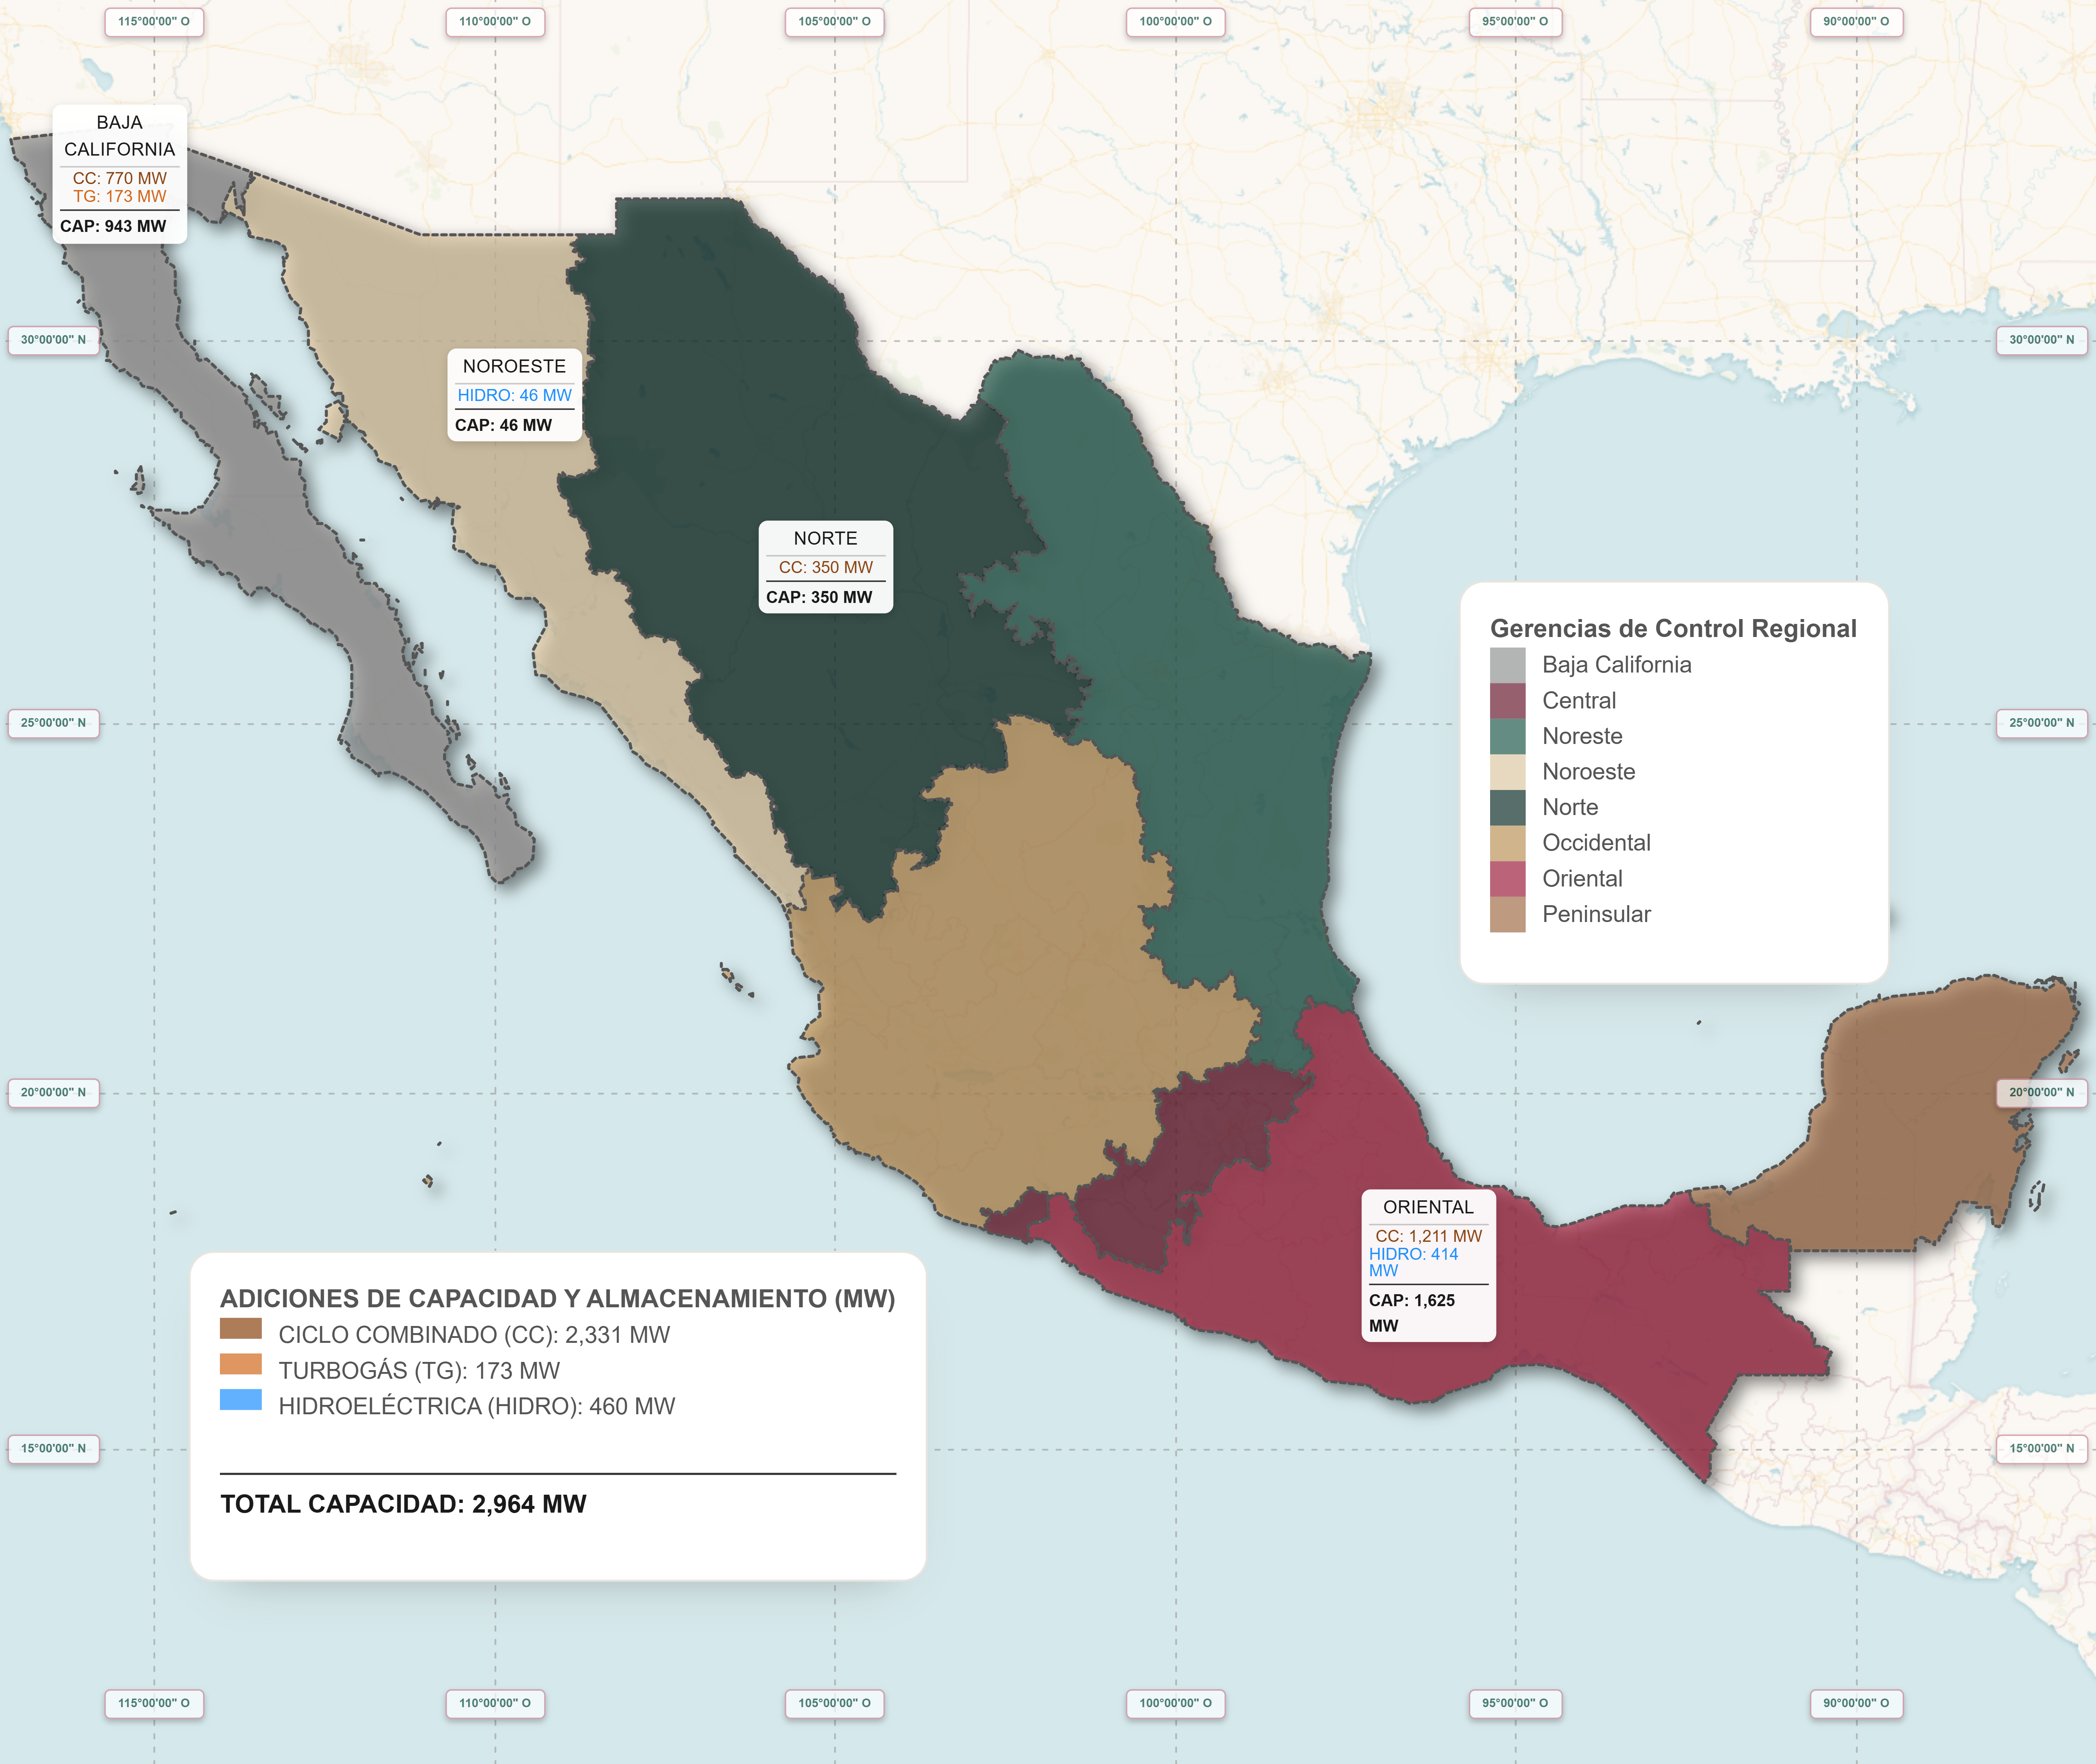
\includegraphics[width=0.8\textwidth]{img/graficos/figura_4_3.png}}{Gráfica de líneas con dos series (solar y eólica) a lo largo de varios años; valores crecientes.}
  \par}
  \raggedright
  \caption{Figura demo: Evolución de capacidad instalada (placeholder)}
  \label{fig:figura_demo__evolucion_de_capa}
\end{figure}
\vspace{-4pt}
\fuente{Elaboración propia

{\fontsize{9pt}{11pt}\selectfont
\begin{itemize}
  \item[\hypertarget{nota1}{1/}] Datos ilustrativos para pruebas
\end{itemize}
}}



\anexos

\section{Ejemplo de anexo}

El primer nivel que contenga 'anexo' debe activar \textbackslash\{\}anexos (numeración alfabética).

\begin{recuadro}[title={Anexo — notas}]
Contenido dentro de anexo.

\end{recuadro}


\subsection{Detalle adicional}

Subanexo (mapea a \textbackslash\{\}subsection en modo anexos).


\section*{Glosario}
\phantomsection
\addcontentsline{toc}{section}{Glosario}

\entradaGlosario{Eficiencia energética}{Relación entre la energía útil obtenida y la energía consumida para lograr un servicio.}
\entradaGlosario{Energías renovables variables}{Tecnologías cuya generación depende del recurso (viento, solar) y fluctúa en el tiempo.}
\entradaGlosario{Flexibilidad del sistema}{Capacidad del sistema eléctrico para responder a variaciones de oferta/demanda, especialmente con renovables variables.}

\printbibliography

\section*{Siglas y Acrónimos}
\phantomsection
\addcontentsline{toc}{section}{Siglas y Acrónimos}

\entradaSigla{CENACE}{Centro Nacional de Control de Energía}
\entradaSigla{CRE}{Comisión Reguladora de Energía}
\entradaSigla{SENER}{Secretaría de Energía}

\paginacreditos{
\begin{center}
{\patriafont\fontsize{12}{14}\selectfont\color{gobmxGuinda} Nombre Apellido Apellido}\\
{\patriafont\fontsize{9}{11}\selectfont Cargo o puesto}\\[0.5cm]
{\patriafont\fontsize{12}{14}\selectfont\color{gobmxGuinda} Nombre 2 Apellido 2}\\
{\patriafont\fontsize{9}{11}\selectfont Cargo 2}\\[0.5cm]
\end{center}
}
\contraportada[img/contraportada.png]{
\textbf{\textcolor{gobmxDorado}{ Elaboración:}}\\
Dirección General (demo)\\[0.5cm]
\textbf{\textcolor{gobmxDorado}{ Contacto:}}\\
correo@ejemplo.gob.mx\\[0.5cm]
\textbf{\textcolor{gobmxGuinda}{ www.gob.mx/sener}}
}

\end{document}
